\documentclass[notes,10pt,aspectratio=169]{beamer}

\usepackage{pgfpages}
% These slides also contain speaker notes. You can print just the slides,
% just the notes, or both, depending on the setting below. Comment out the want
% you want.
\setbeameroption{hide notes} % Only slide
%\setbeameroption{show only notes} % Only notes
%\setbeameroption{show notes on second screen=right} % Both

\usepackage{array}
\usepackage{tgbonum}

% The magic happens here
\usepackage{fontspec}
% \usepackage{lato}
% The magic happens here
\setsansfont[ItalicFont={Fira Sans Italic},%
BoldFont={Fira Sans Bold},%
BoldItalicFont={Fira Sans Italic}]%
{Fira Sans Light}%

\usepackage{tikz}
\usepackage{verbatim}
\setbeamertemplate{note page}{\pagecolor{yellow!5}\insertnote}
\usetikzlibrary{positioning}
\usetikzlibrary{snakes}
\usetikzlibrary{calc}
\usetikzlibrary{arrows}
\usetikzlibrary{decorations.markings}
\usetikzlibrary{shapes.misc}
\usetikzlibrary{matrix,shapes,arrows,fit,tikzmark}
\usepackage{amsmath}
\usepackage{mathpazo}
\usepackage{hyperref}
\usepackage{lipsum}
\usepackage{multimedia}
\usepackage{graphicx}
\usepackage{multirow}
\usepackage{graphicx}
\usepackage{dcolumn}
\usepackage{bbm}
\newcolumntype{d}[0]{D{.}{.}{5}}

\usepackage{changepage}
\usepackage{appendixnumberbeamer}
\newcommand{\beginbackup}{
   \newcounter{framenumbervorappendix}
   \setcounter{framenumbervorappendix}{\value{framenumber}}
   \setbeamertemplate{footline}
   {
     \leavevmode%
     \hline
     box{%
       \begin{beamercolorbox}[wd=\paperwidth,ht=2.25ex,dp=1ex,right]{footlinecolor}%
%         \insertframenumber  \hspace*{2ex} 
       \end{beamercolorbox}}%
     \vskip0pt%
   }
 }
\newcommand{\backupend}{
   \addtocounter{framenumbervorappendix}{-\value{framenumber}}
   \addtocounter{framenumber}{\value{framenumbervorappendix}} 
}

\usepackage{graphicx}
\usepackage[space]{grffile}
\usepackage{booktabs}

\usepackage{verbatim}
\usepackage{ragged2e}
\usepackage{etoolbox}
\apptocmd{\frame}{}{\justifying}{} % Allow optional arguments after frame.

% These are my colors -- there are many like them, but these ones are mine.
\definecolor{blue}{RGB}{0,114,178}
\definecolor{red}{RGB}{213,94,0}
\definecolor{yellow}{RGB}{240,228,66}
\definecolor{green}{RGB}{0,158,115}
\definecolor{crimson}{RGB}{165,28,48}

\hypersetup{
  colorlinks=crimson,
  urlcolor=crimson,
  linkbordercolor = {white},
  linkcolor = {blue}
}

%% I use a beige off white for my background
\definecolor{MyBackground}{RGB}{255,253,218}

%% Uncomment this if you want to change the background color to something else
%\setbeamercolor{background canvas}{bg=MyBackground}

%% Change the bg color to adjust your transition slide background color!
\newenvironment{transitionframe}{
  \setbeamercolor{background canvas}{bg=yellow}
  \begin{frame}}{
    \end{frame}
}

\setbeamercolor{frametitle}{fg=crimson}
\setbeamerfont{frametitle}{series=\bfseries}
\setbeamercolor{title}{fg=black}
\setbeamerfont{title}{series=\bfseries}
\setbeamertemplate{footline}[frame number]
\setbeamertemplate{navigation symbols}{} 
\setbeamertemplate{itemize items}{-}
\setbeamercolor{itemize item}{fg=crimson}
\setbeamercolor{itemize subitem}{fg=crimson}
\setbeamercolor{enumerate item}{fg=crimson}
\setbeamercolor{enumerate subitem}{fg=crimson}
\setbeamercolor{button}{bg=MyBackground,fg=crimson,}


% If you like road maps, rather than having clutter at the top, have a roadmap show up at the end of each section 
% (and after your introduction)
% Uncomment this is if you want the roadmap!
% \AtBeginSection[]
% {
%    \begin{frame}
%        \frametitle{Roadmap of Talk}
%        \tableofcontents[currentsection]
%    \end{frame}
% }
\setbeamercolor{section in toc}{fg=blue}
\setbeamercolor{subsection in toc}{fg=red}
\setbeamersize{text margin left=1em,text margin right=1em} 

\newenvironment{wideitemize}{\itemize\addtolength{\itemsep}{10pt}}{\enditemize}

\usepackage{environ}
\NewEnviron{videoframe}[1]{
  \begin{frame}
    \vspace{-8pt}
    \begin{columns}[onlytextwidth, T] % align columns
      \begin{column}{.70\textwidth}
        \begin{minipage}[t][\textheight][t]
          {\dimexpr\textwidth}
          \vspace{8pt}
          \hspace{4pt} {\Large \sc \textcolor{blue}{#1}}
          \vspace{8pt}
          
          \BODY
        \end{minipage}
      \end{column}%
      \hfill%
      \begin{column}{.38\textwidth}
        \colorbox{green!20}{\begin{minipage}[t][1.2\textheight][t]
            {\dimexpr\textwidth}
            Face goes here
          \end{minipage}}
      \end{column}%
    \end{columns}
  \end{frame}
}

\renewcommand{\appendixname}{\texorpdfstring{\translate{Appendix}}{Appendix}}
% Remove footnote rule
\renewcommand\footnoterule{}

\AtBeginSection{
  \begingroup
  \setbeamercolor{background canvas}{bg=crimson}
  \setbeamercolor{title}{fg=white}
  \setbeamertemplate{footline}{} % Remove page numbering
  \frame{\centering\Large\bf\textcolor{white}{\insertsectionhead}}
  \endgroup
}

\title[]{\textcolor{crimson}{Sesionn 3: RDD}}
\author[RRMRR]{Rony Rodrigo Maximiliano Rodriguez-Ramirez}
\institute[Harvard]{\small{Econ Thaki \\ Harvard University}}
\date{\today}


\begin{document}

%%% TIKZ STUFF
\tikzset{   
        every picture/.style={remember picture,baseline},
        every node/.style={anchor=base,align=center,outer sep=1.5pt},
        every path/.style={thick},
        }
\newcommand\marktopleft[1]{%
    \tikz[overlay,remember picture] 
        \node (marker-#1-a) at (-.3em,.3em) {};%
}
\newcommand\markbottomright[2]{%
    \tikz[overlay,remember picture] 
        \node (marker-#1-b) at (0em,0em) {};%
}
\tikzstyle{every picture}+=[remember picture] 
\tikzstyle{mybox} =[draw=black, very thick, rectangle, inner sep=10pt, inner ysep=20pt]
\tikzstyle{fancytitle} =[draw=black,fill=red, text=white]
%%%% END TIKZ STUFF

% logo of my university
\titlegraphic{
  \includegraphics[width=2cm]{logo/logo_hq.png}\hspace*{4.75cm}~%
  \includegraphics[width=2cm]{logo/harvard-logo.png}
}
% \titlegraphic{
%   \includegraphics[width=2.5cm]{logo/harvard-logo.png}
% }


% Title Slide --------------------------------------------------------------------------------------
\begin{frame}[noframenumbering, plain]
  \maketitle
\end{frame}
% --------------------------------------------------------------------------------------------------

% Diapositiva de contenido
\begin{frame}
  \frametitle{Agenda para hoy}

  En la sesión de hoy, cubriremos:
  \begin{enumerate}
    \item Introducción a Differences-in-Differences (DID)
    \item Configuración Básica del DID
    \item Supuestos e Interpretación
    \item Extensiones del DID
    \item Ejemplos y Demostración en Stata
  \end{enumerate}
\end{frame}

% Diapositiva 1: Introducción al DID
\begin{frame}
  \frametitle{Introducción a Differences-in-Differences (DID)}

  \begin{itemize}
    \item   \textbf{Differences-in-Differences (DID)} es un método cuasi-experimental utilizado para estimar efectos causales comparando los cambios en los resultados a lo largo del tiempo entre un grupo tratado y un grupo de control.

    \vspace{1em}

    \item \textbf{Importancia:}
    \begin{itemize}
      \item Permite controlar por efectos fijos que pueden influir en los resultados.
      \item Útil cuando la asignación aleatoria no es factible, pero hay datos longitudinales.
    \end{itemize}
  \end{itemize}
\end{frame}

% Diapositiva 1: Introducción al DID
\begin{frame}
	\frametitle{DID: Ejemplo de desempleo}

	\begin{figure}\centering
		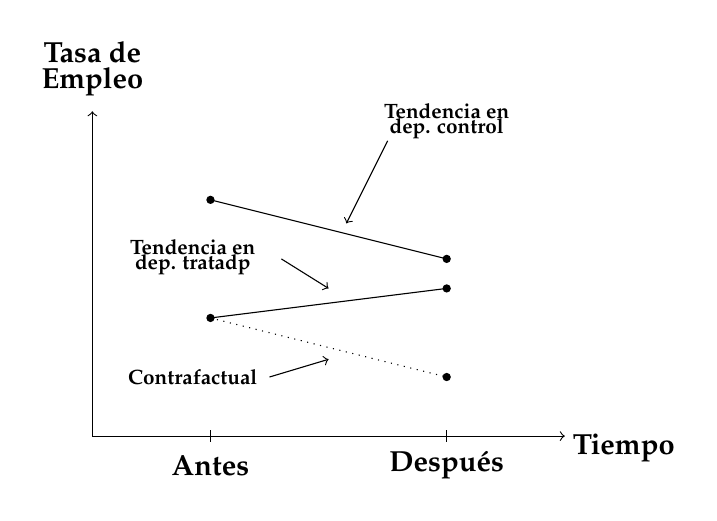
\begin{tikzpicture}[scale=1.5, transform shape]
			%\draw[step=0.5cm,gray,very thin] (0,0) grid (4,3);
			\draw[->] (0,0) -- (4,0) ; 
			\draw[->] (0,0) -- (0,2.75) ; 
			\draw[-] (1,2) -- (3,1.5); 
			\draw[dotted] (1,1) -- (3,0.5); 
			\draw[-] (1,1) -- (3,1.25);
			\draw[->] (2.5,2.5) -- (2.15,1.8);
			\draw[->] (1.6,1.5) -- (2,1.25); 
			\draw[->] (1.5,0.5) -- (2,0.65); 
			\draw[-] (1,0.05) -- (1,-0.05);
			\draw[-] (3,0.05) -- (3,-0.05);
			(3.1,1.25) -- node[right] {{\tiny Efecto}} (3.1,0.5);
			\node at (4.5,-0.1) {\scriptsize\textbf{Tiempo}};
			\node at (0,3.25) {\scriptsize\textbf{Tasa de}};
			\node at (0,3.0) {\scriptsize\textbf{Empleo}};
			\node at (1,-0.25) {\scriptsize\textbf{Antes}};
			\node at (3,-0.25) {\scriptsize\textbf{Después}};
			\node at (3,2.75) {\tiny\textbf{Tendencia en}};
			\node at (3,2.6) {\tiny\textbf{dep. control}};
			\node at (0.85,1.6) {\tiny\textbf{Tendencia en}};
			\node at (0.85,1.45) {\tiny\textbf{dep. tratadp}};
			\node at (0.85,0.5) {\tiny\textbf{Contrafactual}};
			\fill (1,1) circle[radius=1pt];
			\fill (3,0.5) circle[radius=1pt]; 
			\fill (3,1.5) circle[radius=1pt]; 
			\fill (3,1.25) circle[radius=1pt]; 
			\fill (1,2) circle[radius=1pt]; 
		\end{tikzpicture}
	\end{figure} 
\end{frame}

% Diapositiva 2: Configuración Básica del DID
\begin{frame}
  \frametitle{Configuración Básica del DID}

  \textbf{Configuración:} Comparar dos grupos (tratado y control) en dos periodos de tiempo (antes y después del tratamiento).

  \vspace{1em}
  \textbf{Modelo Básico:}
  \begin{itemize}
    \item $Y_{it} = \alpha + \beta_1 \text{Tratamiento}_i + \beta_2 \text{Post}_t + \gamma (\text{Tratamiento}_i \times \text{Post}_t) + \epsilon_{it}$
  \end{itemize}
  donde:
  \begin{itemize}
    \item $Y_{it}$: Resultado para la unidad $i$ en el tiempo $t$
    \item $\text{Tratamiento}_i$: Indicador para el grupo tratado
    \item $\text{Post}_t$: Indicador para el periodo después del tratamiento
    \item $\gamma$: Efecto del tratamiento (DID)
  \end{itemize}
\end{frame}

% Diapositiva 3: Supuestos e Interpretación
\begin{frame}
  \frametitle{Supuestos e Interpretación}

  \textbf{Supuestos Clave:}
  \begin{itemize}
    \item \textbf{Tendencias paralelas:} Las tendencias de resultados habrían sido las mismas en ambos grupos en ausencia de tratamiento.
    \item \textbf{No cambios concomitantes:} No hay eventos coincidentes que afecten de manera diferente a los grupos.
  \end{itemize}

  \vspace{1em}
  \textbf{Interpretación:}
  \begin{itemize}
    \item El coeficiente de interacción $\gamma$ captura el efecto causal del tratamiento.
    \item Es importante verificar gráficamente las tendencias paralelas antes del tratamiento.
  \end{itemize}
\end{frame}

% Diapositiva 4: Extensiones del DID
\begin{frame}
  \frametitle{Extensiones del DID}

  \textbf{DID con Múltiples Periodos:} Extensión que permite evaluar efectos en varios periodos de tiempo.

  \vspace{1em}
  \textbf{DID con Grupos Múltiples:} Permite múltiples grupos tratados con diferentes momentos de inicio del tratamiento.

  \vspace{1em}
  \textbf{DID Dinámico:} Considera cómo el efecto del tratamiento varía con el tiempo desde la intervención.

  \vspace{1em}
  \begin{itemize}
    \item Importante evaluar la robustez de los resultados ante estas extensiones.
  \end{itemize}
\end{frame}

% Diapositiva 5: Lista de Verificación y Ejemplos
\begin{frame}
  \frametitle{Lista de Verificación y Ejemplos}

  \textbf{Lista de Verificación para DID:}
  \begin{itemize}
    \item Verificar el supuesto de tendencias paralelas.
    \item Considerar el uso de covariables adicionales para aumentar la precisión.
    \item Analizar si existen eventos coincidentes que puedan sesgar los resultados.
  \end{itemize}

  \vspace{1em}
  \textbf{Ejemplos:}
  \begin{itemize}
    \item Evaluación del impacto de una reforma laboral sobre el empleo.
    \item Análisis del efecto de un nuevo impuesto sobre el consumo de tabaco.
  \end{itemize}
\end{frame}

% Diapositiva 6: Demostración en Stata
\begin{frame}[fragile]
  \frametitle{Demostración en Stata}

  En Stata, el DID se puede implementar usando comandos como \texttt{reg} o \texttt{xtreg}.

  \vspace{1em}
  \textbf{Código de Ejemplo:}
  
  \begin{verbatim}
    reg Y i.Post##i.Tratamiento, vce(cluster id)
    xtreg Y i.Post##i.Tratamiento, fe vce(cluster id)
    reghdfe Y i.Post##i.Tratamiento, abs(stateid) vce(cluster id)
  \end{verbatim}

  \vspace{1em}
  \textbf{Interpretación de los Resultados:}
  \begin{itemize}
    \item El coeficiente de interacción indica el efecto del tratamiento.
    \item Revisar gráficos de tendencias para validar supuestos.
  \end{itemize}
\end{frame}
% End ----------------------------------------------------------------------------------------------
\end{document}